\documentclass[10pt,twocolumn]{article}
\usepackage[margin=0.75in]{geometry}
\usepackage{times}
\usepackage{graphicx}
\usepackage{booktabs}
\usepackage{amsmath,amssymb}
\usepackage{url}
\usepackage{hyperref}
\usepackage[numbers,sort&compress]{natbib}

\title{Date Night Is a Fragile Institution:\\
Bernoulli Flakes, Hard Quorums, and the\\
Inspection Paradox of Saturday Night}
\author{Ruililin Shen\\
\texttt{bobshenruililin@gmail.com}}
\date{4 September 2026}

% Auto-generated by scripts/make_lonely_numbers.py. Do not edit.

\newcommand{\NumLonelyNOk}{120}
\newcommand{\NumLonelyNFailed}{0}
\newcommand{\NumLonelySeconds}{0.7}
\newcommand{\NumLonelyNSeeds}{5}
\newcommand{\NumLonelyP}{0.70}
\newcommand{\NumLonelyKDyad}{2}
\newcommand{\NumLonelyKDinner}{4}
\newcommand{\NumLonelyKPub}{24}
\newcommand{\NumLonelyAloneDyad}{0.510}
\newcommand{\NumLonelyAloneDinner}{0.319}
\newcommand{\NumLonelyAlonePub}{0.300}
\newcommand{\NumLonelyDeltaExact}{0.210}
\newcommand{\NumLonelyDeltaDinner}{0.019}
\newcommand{\NumLonelyExtraDyad}{0.210}
\newcommand{\NumLonelyExtraPub}{0.000}
\newcommand{\NumLonelyFloor}{0.300}
\newcommand{\NumLonelyKillDelta}{0.000}
\newcommand{\NumLonelyKillDyad}{0.300}
\newcommand{\NumLonelyKillPub}{0.300}
\newcommand{\NumLonelyQualityExact}{0.210}
\newcommand{\NumLonelyDeltaMc}{0.212}
\newcommand{\NumLonelyDeltaMcStd}{0.003}
\newcommand{\NumLonelyDyadMc}{0.511}
\newcommand{\NumLonelyPubMc}{0.299}
\newcommand{\NumLonelyQualityMc}{0.209}
\newcommand{\NumLonelyQualityMcStd}{0.001}
\newcommand{\NumLonelyInspAtt}{2.943}
\newcommand{\NumLonelyInspAttStd}{0.010}
\newcommand{\NumLonelyInspEvent}{1.122}
\newcommand{\NumLonelyFeedAtt}{10.865}
\newcommand{\NumLonelyFeedEvent}{4.143}
\newcommand{\NumLonelyProposed}{3.7}
\newcommand{\NumLonelyShareOutLarge}{0.587}
\newcommand{\NumLonelySharePeopleLarge}{0.500}
\newcommand{\NumLonelyFomoAtt}{7.173}
\newcommand{\NumLonelyCompareStay}{10.9}
\newcommand{\NumLonelyCompareSmallOut}{8.9}
\newcommand{\NumLonelyDyadCancel}{0.511}
\newcommand{\NumLonelyPubCancel}{0.000}
\newcommand{\NumLonelyKillMcDelta}{-0.001}
\newcommand{\NumLonelyKillMcStd}{0.001}
\newcommand{\NumLonelyRhoDelta}{0.140}
\newcommand{\NumLonelyRhoDeltaStd}{0.004}
\newcommand{\NumLonelyMatchN}{6}
\newcommand{\NumLonelyMatchAlone}{0.302}
\newcommand{\NumLonelyOverbookAlone}{0.302}
\newcommand{\NumLonelyOverbookN}{6}
\newcommand{\NumLonelyFrailtyDyadIndep}{0.510}
\newcommand{\NumLonelyFrailtyDyadCorr}{0.445}
\newcommand{\NumLonelyFrailtyPubCorr}{0.303}
\newcommand{\NumLonelyNPeople}{2400}
\newcommand{\NumLonelyNNights}{30}


\begin{document}
\maketitle
\begin{abstract}
Wanting one other person---a date, a catch-up, ``quality time''---is a
statistically lonely desire. Each invitee shows independently with
probability $p$; the gathering happens iff at least $q$ people arrive.
A person is not alone iff they show \emph{and} the gathering happens.
At $q=2$ and $p=\NumLonelyP$, the closed-form chance of a night alone is
$\NumLonelyAloneDyad$ for a dyad ($k=\NumLonelyKDyad$) versus
$\NumLonelyAlonePub$ for a pub ($k=\NumLonelyKPub$): extra isolation
$\NumLonelyDeltaExact$ above the own-flake floor $1-p=\NumLonelyFloor$.
The $q=1$ kill is exact zero: if showing up to an empty table counts,
dyads and pubs are identical. Monte Carlo on
$\NumLonelyNPeople$ numpy people $\times$ $\NumLonelyNNights$ nights
$\times$ $\NumLonelyNSeeds$ seeds matches
($\Delta=\NumLonelyDeltaMc\pm\NumLonelyDeltaMcStd$).
Replacing pubs with dyads, same person-slots, raises population nights-alone
by $\NumLonelyQualityExact$. In a 50/50 mix, most \emph{events} are dates
(mean proposed size $\NumLonelyProposed$) but the attendance-weighted feed
is a pub (mean $\NumLonelyFeedAtt$, ratio $\NumLonelyInspAtt$).
Airline-overbooking a date to $\NumLonelyMatchN$ people approaches the
flake floor and ceases to be a date. This is a generative cartoon, not a
UCLA survey and not a measurement of the loneliness epidemic.
\end{abstract}

\section{Laugh, then think}

The laugh: the statistically honest cure for a cancelled Friday is to
triple-book the other person, or to go where cancellation is impossible---the
pub. The think: intimacy and flake-robustness are binomial-incompatible
under independent shows. A society that moves social life from large,
low-quorum rooms (pubs, churches, clubs) into one-on-one catch-ups can
raise nights-alone \emph{without anyone becoming less willing to show up}.

Isolation is associated with mortality risk~\cite{holtlunstad2015mortality}.
Loneliness is not the same thing as isolation: it is a subjective gap
between desired and achieved contact~\cite{cacioppo2010loneliness,hughes2004short,russell1980ucla}.
We do not collect those scales. We measure a mechanical source of the
gap: nights alone, and a Saturday-night feed that over-represents surviving
crowds.

\section{What this is not}

Feld's friendship paradox---your friends have more friends than you
do---is length-biased sampling on
degree~\cite{feld1991friends,jackson2019friendship}. So are the happiness
paradox~\cite{bollen2017happiness} and the majority
illusion~\cite{lerman2016majority}. Feld already noted that beaches feel
more crowded than they ``usually'' are. We do not retitle that.

Group-chat folklore already knows that flakes kill small plans. The
identifying pieces here are (i)~a closed form,
(ii)~a $q=1$ kill that isolates quorum from ``people got flakier,''
(iii)~a quality-over-quantity comparative static at fixed person-slots,
(iv)~survivorship plus inspection of the feed, and (v)~a copula that
holds the marginal show-up rate fixed.

Granovetter thresholds make attendance a strategic complement: you go if
enough others go~\cite{granovetter1978threshold}. Our people are worse
and simpler. They flip independent coins. Small gatherings still collapse.

Social-media FOMO is a human measurement~\cite{hunt2018fomo}. Our ``feed''
is just happening events, weighted by how many people were there to post.

\section{Model}

$k$ invitees, including you. Each shows independently with probability
$p$. Quorum $q$. You attend a happening event iff you show and at least
$q-1$ of the others show:
\begin{equation}
  P(\mathrm{attend})=
  \begin{cases}
    p & q\le 1,\\
    p\cdot P\bigl(\mathrm{Bin}(k-1,p)\ge q-1\bigr) & q\ge 2.
  \end{cases}
\end{equation}
$P(\mathrm{alone})=1-P(\mathrm{attend})$. The own-flake floor is $1-p$:
a stadium cannot socialize a person who stays home. Extra isolation above
that floor is $p\cdot P(\mathrm{Bin}(k-1,p)<q-1)$. For the pair quorum
$q=2$ this is exactly $p(1-p)^{k-1}$: everyone else flaked.

\textbf{H1.} At $q=2$ and $p\in(0,1)$,
$\Delta_{\mathrm{alone}}=P(\mathrm{alone}\mid k=2)-P(\mathrm{alone}\mid k=24)>0$.

\textbf{Kill H1.} $q=1$ $\Rightarrow$ $\Delta_{\mathrm{alone}}=0$.

\textbf{H2/H3.} In a mixed calendar of dyads and pubs, cancelled dates
vanish and remaining person-nights length-bias toward pubs, so the
attendance-weighted feed exceeds the event-weighted proposed mean.

\textbf{Policy.} Convert every pub into dyads (same slots): population
$P(\mathrm{alone})$ rises. Over-invite a dyad until it matches the pub:
it is no longer a dyad.

\section{Protocol}

Exact binomial identities for $k\in\{2,3,4,6,8,12,24,48\}$,
$p\in\{0.5,0.6,0.7,0.8\}$, quorum rules $\{\texttt{one},\texttt{pair},\texttt{half}\}$.
Finite-population calendars: $\NumLonelyNPeople$ people,
$\NumLonelyNNights$ nights, $\NumLonelyNSeeds$ seeds, no double booking.
Headline cell: $p=\NumLonelyP$, $q=2$, latent correlation $\rho=0$.
Robustness: Gaussian copula $\rho=0.5$ with Bernoulli($p$) margins
(unlike a logit shock, this does not move $E[p]$).
JSON: \texttt{results/exp10\_quorum\_lonely.json}
($\NumLonelyNOk$ cells ok, $\NumLonelyNFailed$ failed,
$\NumLonelySeconds$\,s). No hand-edited numbers.

\section{Results}

\paragraph{H1, exact.}
Figure~\ref{fig:alonek} plots $P(\mathrm{alone})$ against $k$. At $q=2$,
$p=\NumLonelyP$, a dyad is alone with probability $\NumLonelyAloneDyad$,
a four-person dinner $\NumLonelyAloneDinner$, a pub
$\NumLonelyAlonePub$. Extra isolation is $\NumLonelyExtraDyad$ versus
$\NumLonelyExtraPub$. The dinner is almost a pub; the date is not.
Monte Carlo: $\Delta=\NumLonelyDeltaMc\pm\NumLonelyDeltaMcStd$
(dyad $\NumLonelyDyadMc$, pub $\NumLonelyPubMc$).
Dyad cancellation rate $\NumLonelyDyadCancel$; pub cancellation
$\NumLonelyPubCancel$.

\paragraph{Kill.}
$q=1$: exact $\Delta=\NumLonelyKillDelta$ (both equal the flake floor
$\NumLonelyKillDyad$). MC $\Delta=\NumLonelyKillMcDelta\pm\NumLonelyKillMcStd$.
If an empty table counts as company, wanting a date is no lonelier than
wanting a crowd. The loneliness of the dyad \emph{is} the refusal to count
that table.

\paragraph{Quality-over-quantity.}
Turning pubs into dyads raises nights-alone by $\NumLonelyQualityExact$
exact, $\NumLonelyQualityMc\pm\NumLonelyQualityMcStd$ MC
(Figure~\ref{fig:kill}). Same invitations, same $p$, more isolation.

\paragraph{The feed (H3).}
Half the people are assigned dates, half pubs. The \emph{event} calendar
is almost all dates (mean proposed size $\NumLonelyProposed$). Happening
events are only slightly larger ($\NumLonelyFeedEvent$, ratio
$\NumLonelyInspEvent$) because cancelled dates drop out. Weight by
attendees---the Instagram of Saturday night---and the mean jumps to
$\NumLonelyFeedAtt$ (ratio $\NumLonelyInspAtt$;
Figure~\ref{fig:fomo}). Stay-homes compare an empty room to a feed of
size $\NumLonelyCompareStay$. People whose date \emph{happened} still
see a feed $\NumLonelyCompareSmallOut$ larger than their table.
Pub people are $\NumLonelySharePeopleLarge$ of the population but
$\NumLonelyShareOutLarge$ of person-nights out.

\paragraph{Overbooking.}
The smallest $n$ that matches the pub within $0.005$ is
$\NumLonelyMatchN$ (alone $\NumLonelyMatchAlone$;
Figure~\ref{fig:over}). Inviting $\NumLonelyOverbookN$ at $m=3$ gives
$\NumLonelyOverbookAlone$. It works. It is not a date.

\paragraph{Correlated Friday nights.}
Shared latent correlation $\rho=0.5$ (fixed marginal $p$) helps dyads:
alone $\NumLonelyFrailtyDyadCorr$ versus $\NumLonelyFrailtyDyadIndep$ independent;
pubs stay at $\NumLonelyFrailtyPubCorr$. MC $\Delta$ shrinks to
$\NumLonelyRhoDelta\pm\NumLonelyRhoDeltaStd$ but does not die.
Independence is the worst case for date night, not the only case.

\begin{figure}[t]
\centering
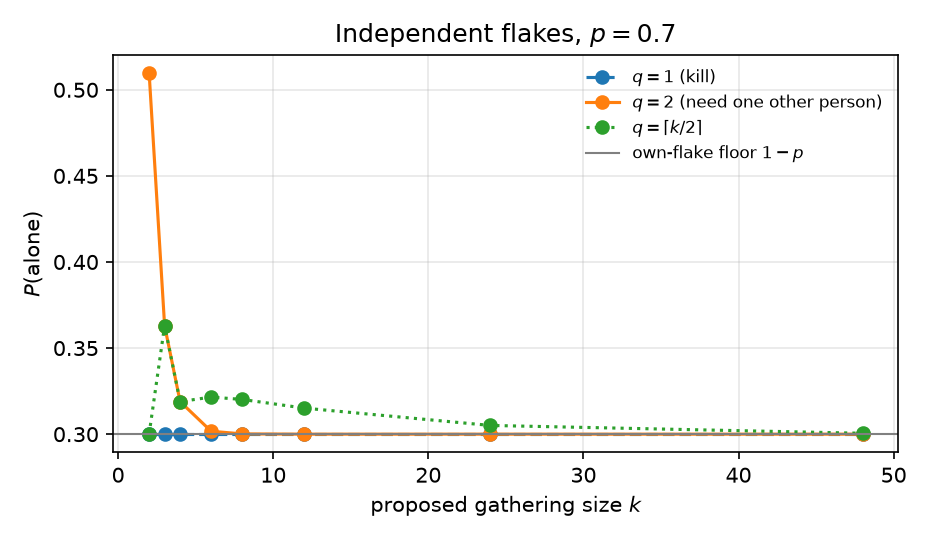
\includegraphics[width=\columnwidth]{../figures/png/lonely_alone_vs_k.png}
\caption{$P(\mathrm{alone})$ versus proposed size. The $q=1$ curve is
the flake floor. Pair quorum makes small $k$ uniquely expensive.
\label{fig:alonek}}
\end{figure}

\begin{figure}[t]
\centering
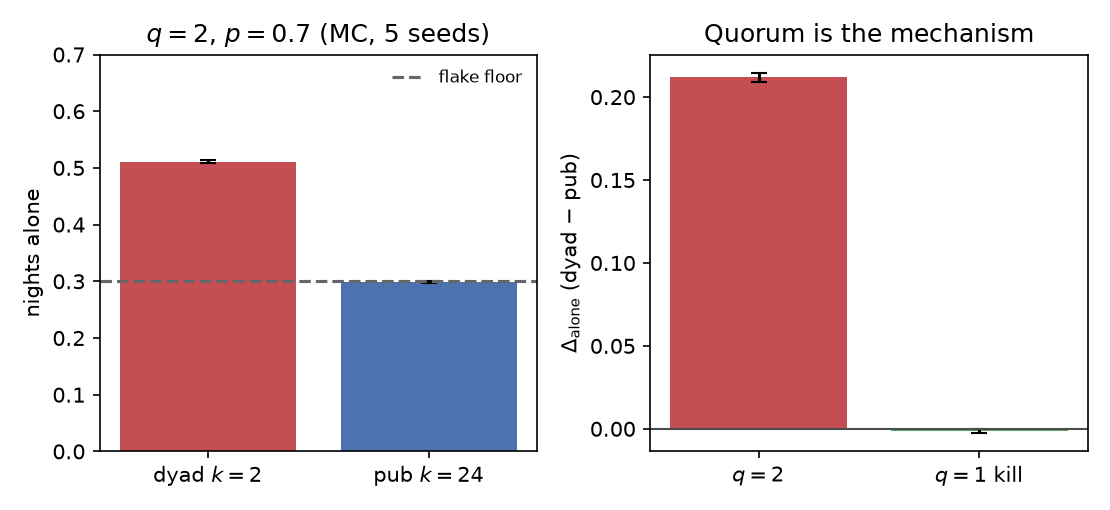
\includegraphics[width=\columnwidth]{../figures/png/lonely_quality_kill.png}
\caption{Left: nights alone, dyad versus pub. Right: $\Delta_{\mathrm{alone}}$
dies at $q=1$. Error bars are seed sd ($n=\NumLonelyNSeeds$).
\label{fig:kill}}
\end{figure}

\begin{figure}[t]
\centering
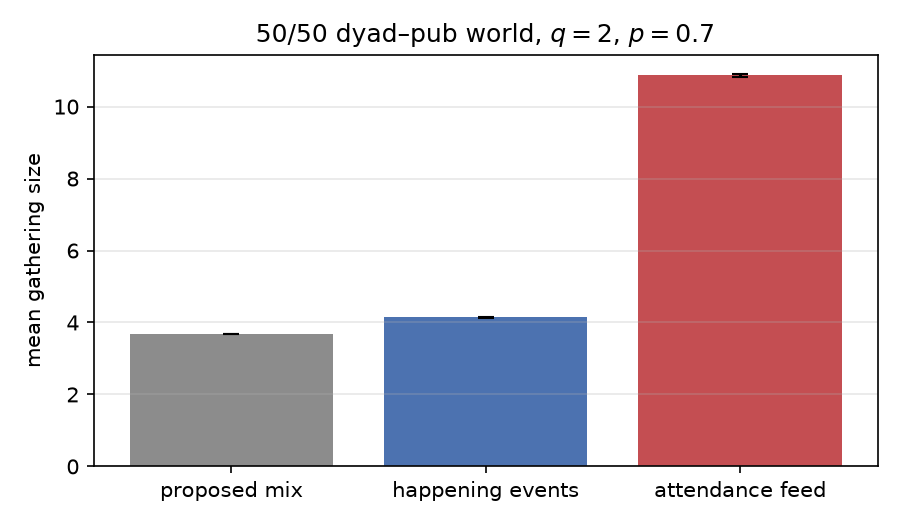
\includegraphics[width=\columnwidth]{../figures/png/lonely_fomo_feed.png}
\caption{50/50 dyad--pub world. Most events are small; most attendances
are not.\label{fig:fomo}}
\end{figure}

\begin{figure}[t]
\centering
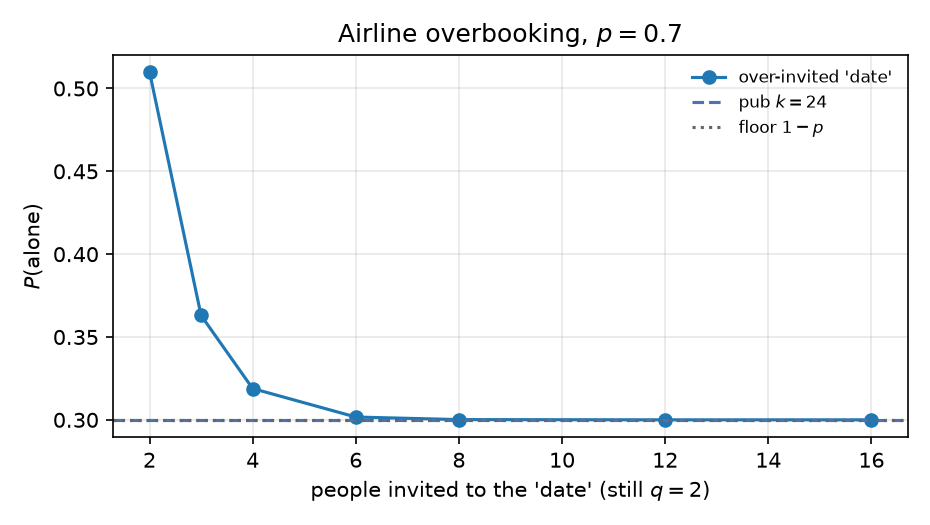
\includegraphics[width=\columnwidth]{../figures/png/lonely_overinvite.png}
\caption{Over-inviting a ``date'' approaches the pub and the flake floor
by ceasing to be a date.\label{fig:over}}
\end{figure}

\section{Limitations}

Numpy people. No ATUS, no GSS, no IRB, no UCLA items. $p$ is a cartoon of
RSVP/flake, not a fitted no-show rate. Real availability is more structured
than an equicorrelated probit. Hosts are not strategic; nobody reschedules.
We do not claim the loneliness epidemic is ``just math,'' and we do not
recommend triple-booking humans. The result is an identifying DGP: if
social contact is implemented as small-$k$ coordination with independent
flakes and a hard quorum of two, nights-alone rise relative to large
low-quorum rooms \emph{even when willingness to show up is unchanged}.

\section{Conclusion}

Date night is a fragile institution. Pubs are not. A feed that samples
people who went out will look like a pub even when the calendar is dates.
The Ig Nobel policy is grotesque on purpose: invite extra people you did
not want, or sit where cancellation cannot find you. The serious reading
is narrower. ``Quality over quantity,'' implemented as a shift from
flake-robust rooms to dyads, is a binomial tax on contact.

\bibliographystyle{unsrtnat}
\bibliography{lonely_verified}
\end{document}
